\section{Introduction}

Recently, procedure planning has exhibited critical reasoning capability for solving real-world challenges in complex domains, such as robotic navigation~\citep{sermanet2024robovqa,bhaskara2024trajectory} and autonomous driving~\citep{wang2024driving,liao2024bat}. 
Among them, procedure planning in instructional videos~\citep{zhao2022p3iv,wang2023pdpp,li2023skip} has been widely concerned because of its wide application scenarios, which involve identifying and generating coherent action sequences that align with the task's objectives, given the start and end visual observations.

% 说明各个方法的核心
In the field of procedure planning in instructional videos, the primary challenge lies in modeling the temporal evolution mechanism among actions and identifying pertinent conditions that can effectively steer the generation of intermediary actions in scenarios where information is scarce. 
As depicted in \Cref{fig:task}(a), many scholars have resorted to capturing different forms of auxiliary information about the intermediate states to bridge the gap between observed states and unobserved actions. 
% example
For example, event-based supervision~\citep{wang2023event} leverages key task events to help the model learn temporal action structures, while task label supervision~\citep{wang2023pdpp} uses task-specific labels for better alignment with the task objective. The probabilistic procedure knowledge graph~\citep{nagasinghe2024not} provides structured knowledge to enhance the understanding of action dependencies. Additionally, \citet{niu2024schema} leverage large language models (LLMs) to describe state changes, improving the model’s grasp of causal relationships by combining visual and language descriptions.
% problem
%However, these methods rely on text-level supervision instead of visual-level feature supervision, leading to less detailed and comprehensive information. 
However, all these methods are limited to providing text-level supervision, resulting in less detailed and comprehensive information, and failing to precisely capture the temporal relationships between actions. 
Additionally, these methods decouple the acquisition of supervisory information from the intermediate action reasoning process, hindering effective collaboration and interaction between the two. Consequently, it becomes challenging to fully integrate and adapt to current action reasoning tasks. 

%In light of these discrepancies, we investigate reconstructing and complementing the mid-state visual supervision by computing the temporal logical relationships between actions.

\begin{figure}[t]
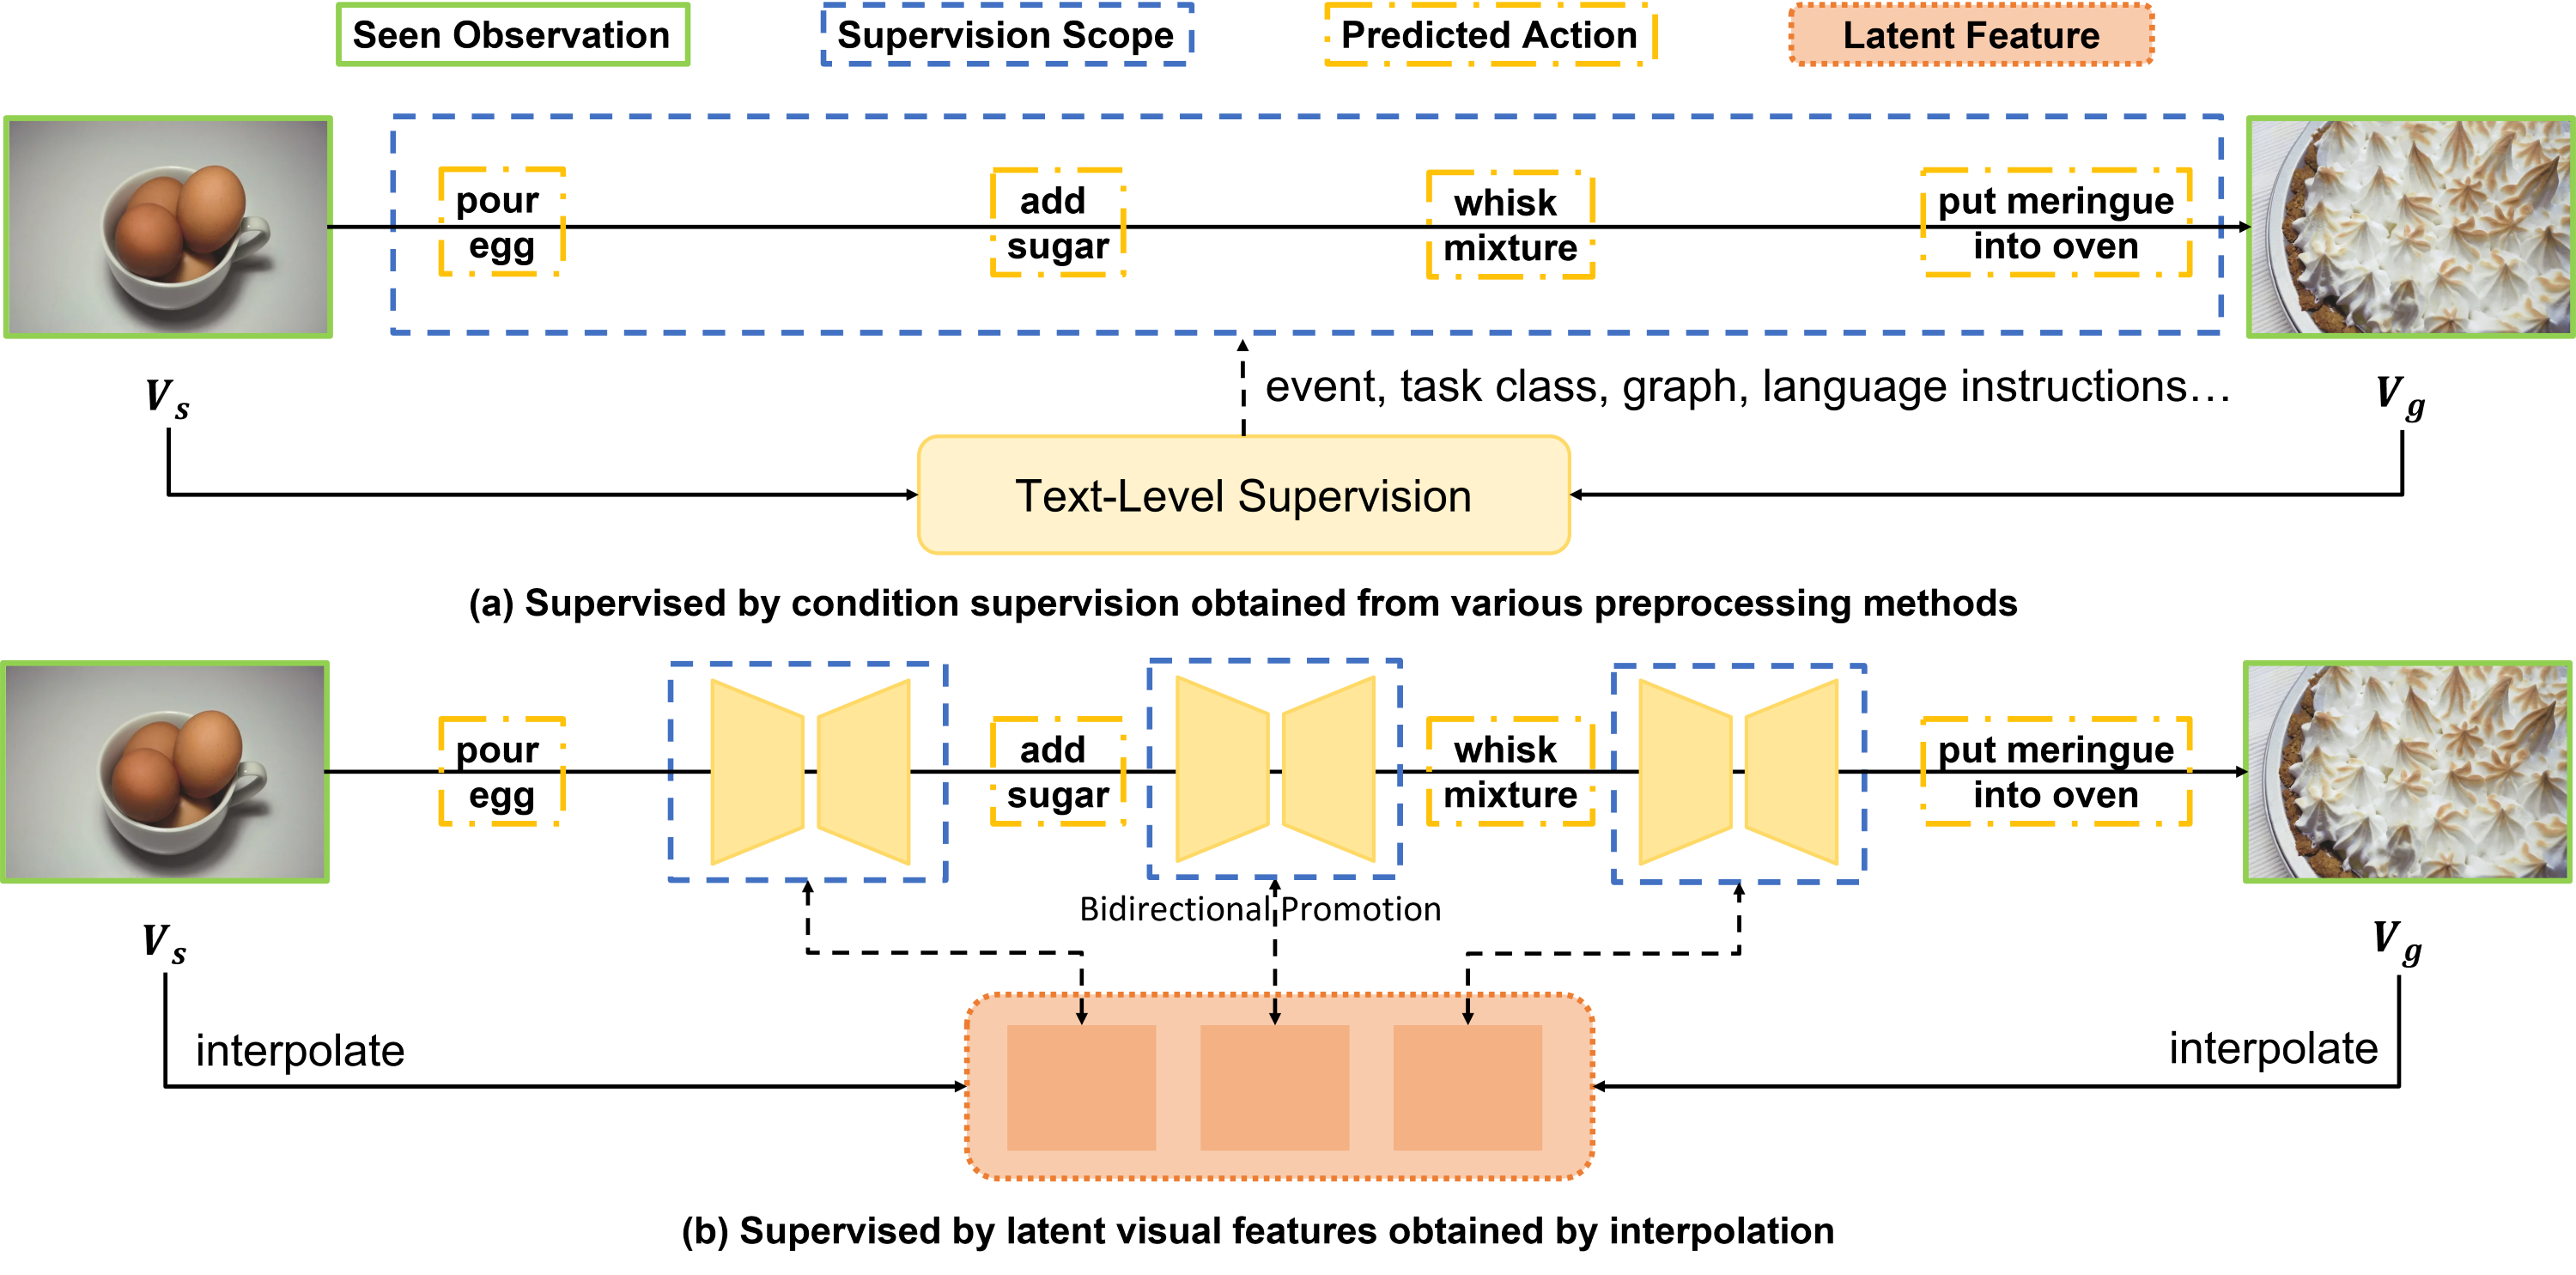
\includegraphics[width=0.98\textwidth, keepaspectratio]{figures/fig-task.png}
% \vspace{-0.5em}
\caption{The core idea to solve procedure planning with previous methods and ours. }
\label{fig:task}
% \vspace{-2.5mm}
\end{figure}

%%%%%%%%%%%
% 这个是一个总括,波波倒数第二段
%%%%%%%%%%%%
Based on the above analysis, we propose the Masked Temporal Interpolation Diffusion (MTID) model for procedure planning in instructional videos. 
As shown in \Cref{fig:task}(b), the core concept is to leverage intermediate latent visual features, generated synchronously by a latent space temporal logical interpolation module, to provide comprehensive visual-level information for mid-state supervision. 
In the meanwhile, the generated visual features are directly injected into the action reasoning model, ensuring the generation of intermediate supervision information can be effectively applied to the current action reasoning task through end-to-end training.

%%%%%%%%%%%%%%
% 总结我们的主要贡献
%%%%%%%%%%%
% 构成
Specifically, \textbf{MTID} consists of three core components: a task classifier, a latent space temporal logical interpolation module, and a diffusion model framework that incorporates both a U-Net and a DDIM strategy.
% first
In the first stage, a transformer-based classifier predicts the task class label $c$ for the entire instructional video, given the start and end observations. This prediction serves as the foundation for subsequent reasoning and action generation.
% second
The latent space temporal logical interpolation module is designed to capture and model temporal relationships. 
% 1
It employs an observation encoder to transform the visual features of the observations into latent features that maintain temporal dependencies and discard object details. 
% 2
A latent space interpolator then generates intermediate features using a learnable interpolation matrix, which dynamically adjusts the interpolation ratio to fit task-specific requirements. 
% 3
These interpolated features are refined through transformer blocks, enhancing their temporal coherence and capturing the dependencies between action sequences.
% third
In the third stage, during the denoising phase for generating action sequences, the input matrix is constructed by concatenating the task class label, observed visual features, and Gaussian noise sampled from $\mathcal{N}(0, I)$. 
% mask
A masked projection is applied to exclude irrelevant actions, ensuring that the generated actions remain within the desired range. 
% ddim
To accelerate inference, DDIM is used throughout the iterative process.
% loss
To further ensure task relevance, a task-adaptive masked proximity loss is introduced. This loss function gradually decreases its focus toward the central features, reinforcing supervision on intermediate latent features while penalizing irrelevant actions, thereby constraining the generation process. 
% all
By leveraging detailed information from both the start and end observations $V_s$ and $V_g$, our model accurately predicts target action sequences, as demonstrated by experimental results on the CrossTask, COIN, and NIV datasets.

The main contributions of this paper are as follows:
\begin{itemize}[leftmargin=*]
%\vspace{-2mm}
    \item We propose a Masked Temporal Interpolation Diffusion model with a mask to limit action initialization and a task-adaptive masked proximity loss to enhance accuracy.
    
    \item We use a latent space temporal logical interpolation module to extract intermediate visual features with temporal relationships from the start and end states to guide the diffusion process.
    
    \item Extensive experiments are conducted on several widely used benchmarks, showing significant performance improvements on multiple tasks using the proposed method.
\end{itemize}




% Specifically, \textbf{MTID} consists of a transformer-based classifier, a latent space temporal logical interpolation module, and a diffusion model framework, which includes a U-Net and a DDIM strategy. Given a start observation $V_s$ and a goal observation $V_g$, the transformer-based classifier assigns the corresponding task labels $c$ for task supervision. For the latent space temporal logical interpolation module, the observation encoder $E$ transforms the input observations $V_s$ and $V_g$ into latent features $L_s$ and $L_g$, converting the visual features with object details into logical features with temporal relationships. The interpolator then generates intermediate latent features $I_{1:M}$ by applying a learned interpolation matrix $\phi$, dynamically adjusting the interpolation ratio to adapt to different tasks. These latent features are further refined through transformer encoder blocks $TF$, producing intermediate features $F_{1:M}$, with additional temporal logical information. Next, concatenating noise $\varepsilon_{1:T} \sim \mathcal{N}(0, I)$, the task label $c$, and the observations $V_s$ and $V_g$ into the matrix $\hat{x}_N$, we apply a masked projection to $\hat{a}_{1:T}$ during initialization to restrict irrelevant actions during iteration. This is then input into the U-Net model $f_\theta$ to fit the distribution of the target actions $a_{1:T}$. During this process, $F_{1:M}$ is incorporated via cross-attention to assist in the fitting. A task-adaptive masked proximity loss $\mathcal{L}_{\mathrm{diff}}$ is also applied to strengthen supervision of the intermediate latent features and penalize actions that do not align with the task. Consequently, with the detailed information from $V_s$ and $V_g$, the model can predict target action sequences, as demonstrated across various datasets.

% 太细节化  流程化了   讲了一遍方法的流程  没啥意思
% 讲你那插值   mask和loss的目的  核心思想   好处就行    让人明白最high-level的东西
